\documentclass[11pt, a4paper, oneside]{ctexart}
\usepackage{amsmath, amsthm, amssymb, appendix, bm, graphicx, hyperref, mathrsfs}
\usepackage{fancyhdr}%导入fancyhdr包
\usepackage{ctex}%导入ctex包
\usepackage{animate}
\usepackage{geometry}
\usepackage{cite}
\usepackage{setspace}
\usepackage{graphicx}
\usepackage{pythonhighlight}
\usepackage{scalerel}
\usepackage{listings}
\usepackage{ctex}
\usepackage{graphicx}
\usepackage{setspace}
\usepackage{amsthm,amsmath,amssymb}
\usepackage{mathrsfs}
%\usepackage[a4paper, body={18cm,22cm}]{geometry}

\usepackage{float,abstract,booktabs,indentfirst,amsmath}
\usepackage{array}
\usepackage{booktabs} %调整表格线与上下内容的间隔
\usepackage{multirow}
\usepackage{url}
\usepackage{diagbox}
\renewcommand\arraystretch{1.4}
\usepackage{indentfirst}
\setlength{\parindent}{2em}

\usepackage{listings}
\usepackage{xcolor}

\renewcommand{\baselinestretch}{1.5}
%\geometry{left=2.8cm,right=2.8cm,top=2.5cm,bottom=2.5cm}
%\geometry{left=3.18cm,right=3.18cm,top=2.54cm,bottom=2.54cm}
\geometry{left=3.10cm,right=3.18cm,top=3.14cm,bottom=2.5cm}

\pagenumbering{arabic}%设置页码格式,大写字母标页
\pagestyle{fancy}
\fancyhead{} % 初始化页眉
\fancyhead[R]{\small{王治平\ 320200908151}}
\fancyhead[L]{\small{微振动系统的本征振动频率与模式的数值计算探究}}
\fancyfoot{} % 初始化页脚
%\fancyfoot[LO]{奇数页左页脚}
%\fancyfoot[LE]{偶数页左页脚}
%\fancyfoot[RO]{奇数页右页脚}
%\fancyfoot[RE]{偶数页右页脚}
\fancyfoot[R]{\thepage}
\renewcommand{\headrulewidth}{0.8pt}%分隔线宽度4磅
\renewcommand{\footrulewidth}{0pt}
\title{\textbf{微振动系统的本征振动频率与模式的数值计算探究
}}
\begin{spacing}{0}

\author{{王治平} 
\\\vspace{-6mm}
\small{2020级\ \ 物理学二班}
\\\small{320200908151}
\\{指导老师:吴枝喜、关剑月}}
    %%行间距变为double-space
\end{spacing} 
\date{\today}
\linespread{1.5}
\newtheorem{theorem}{定理}[section]
\newtheorem{definition}[theorem]{定义}
\newtheorem{lemma}[theorem]{引理}
\newtheorem{corollary}[theorem]{推论}
\newtheorem{example}[theorem]{例}
\newtheorem{proposition}[theorem]{命题}
\renewcommand{\abstractname}{\Large\textbf{ }}




\begin{document}
\maketitle
	%\tableofcontents
	
	%\begin{center}
		%\LARGE{{\textbf{\heiti 实验一 远程过程调用中间件及数据访问中间件}}}
		%\newline
		%\newline
		%\date{2019年4月2日}
		%\begin{table}[H]
		%	\centering
		%	\begin{tabular}{p{3cm}p{4cm}<{\centering}p{3cm}p{4cm}<{\centering}}
		%		班\quad 级: & 2020级物理学一班 & 学\qquad 号:   & 320200908151 \\ \cline{2-2} \cline{4-4}
		%		姓\quad 名: & 王治平       & 指导老师: &吴枝喜、关剑月       \\ \cline{2-2} \cline{4-4} 
		%	\end{tabular}
		%\end{table}
	%\end{center}

    \maketitle

    \setcounter{page}{0}
    \maketitle
    \thispagestyle{empty}
    ~\\~\\~\\

\maketitle

\setcounter{page}{0}
\maketitle
\thispagestyle{empty}

\begin{abstract}
    {\setlength{\parindent}{0em}\textbf{摘要:}\emph{
    微振动系统的本征频率和本征模式问题已有不少人讨论过,
    本次课题首先复现出他人做过的五自由度的微振动问题
    ,之后进行推广,得到任意自由度的数值计算结果。之后尝试与
    理论数据比较,进行理论和算法的改进与修正
    入手,复现出网站的进展,接下来进行理论推广,得到了
    多自由度的微振动系统的本征问题的数值计算。期间进行了时间复杂度的
    多次优化和算法改进,同时就对称性进行了讨论。本文最后给出了结果较为理想
    的数值计算思路与数值结果,同时给出对应的解析解,并指出了
    部分的优化算法思路与实现。
    }


    }
    \vspace{6mm}
    \setlength{\parindent}{2em}\textbf{关键字:}{微振动系统,解析求解,对比,本征问题,多自由度
    ,$python$,近似选取,算法优化}
\end{abstract}

\vspace{30mm}\begin{center}
    \small{课题程序实现已上传}\small{\\$\quad https://github.com/YingD0/level2/tree/main/work2$}
        
\end{center}

\newpage
\pagenumbering{Roman}
\setcounter{page}{1}
\tableofcontents
\newpage
\setcounter{page}{1}
\pagenumbering{arabic}

\section{课题介绍}
\subsection{课题介绍}
{
    $\bullet$\textbf{微振动系统}


    \setlength{\parindent}{3em}{振动是指系统对于平衡位形的某种
    周期性偏离。而微振动是指这种偏移量极小的振动。一般情况下的处
    理方法列出力学方程之后进行简谐近似来进行处理分析。}


    \setlength{\parindent}{2em}$\bullet$\textbf{本征振动频率与模式}


    \setlength{\parindent}{3em}对于一个多自由度的微振动系统
    ,我们可以选取系统自由度的适当线性组合构成简正坐标(又称简正模),这些简正坐标
    的简谐振动是互相独立的,其相应的,由力学性质与参数决定
    的频率被称为本征振动频率(又称作本征频率)。

}
\subsection{课题简介}
{本课题旨在对一种简单的无阻尼五自由度系统的振动进行简要分析\footnote{本项目中提到的五自由度系统来源于资料1}的振动能级进行数值
计算,期间用到了一些力学基础知识以及线性代数以及数值计算技巧,并对与结果进行了相关讨论。}
\newpage
\section{理论分析}
\subsection{一般性原理介绍}
\subsubsection{分析步骤}
{本课题的目的是分析系统的振动模式与频率,一般来讲对于一般的
微振动我们可以按照如下步骤进行理论分析。\cite{h}

\textbf{(\romannumeral1)写出体系的拉格朗日量}

\textbf{(\romannumeral2)对体系能量进行简谐近似}

\textbf{(\romannumeral3)将近似之后的拉格朗日量代入拉格朗日方程}


$\qquad${一般情况下,由于自由度之间的耦合我们得到的运动方程较为复杂,方便起见

$\qquad$一般会对方程进行一些可控变换达到脱耦}

\textbf{(\romannumeral4)用傅里叶变换或者二次型对角化方法脱耦}

\textbf{(\romannumeral5)利用脱耦之后的拉格朗日方程,求出本征频率与简正模}

\textbf{(\romannumeral6)结合给出的初始条件,计算出每个简正模式的贡献,得出运动方程}




\subsubsection{自由度为s情况的分析}

以上步骤陈列过于泛泛,实际价值不高,下面我们
以自由度为s的情况进行具体分析:\cite{h}\cite{i}

\textbf{(\romannumeral1)写出体系的拉格朗日量}

按照惯例用$q_i$表示广义坐标,$a_{ij}$表示动能系数,对于一般的保守系,系统的势能$U$是且
仅是$q_i(i=1,2,3,4\dots,s)$的函数,
故动能可以写作:
\begin{equation}
    T = \frac{1}{2}\sum_{i,j}a_{ij}(q)\dot{q_i}\dot{q_j} 
\end{equation}
拉格朗日量$\mathscr{L}$可写作
\begin{equation}
    \mathscr{L} = \frac{1}{2}\sum_{i,j}a_{ij}(q)\dot{q_i}\dot{q_j} -U(q)
\end{equation}

\textbf{(\romannumeral2)对体系能量进行简谐近似}

由微振动的定义,
$U$在$q_i = q_{i0}$处取极小,同时可以将偏离平衡位置的
小位移表示为:
\begin{equation}
    x_i = q_i - q_{i0}
\end{equation}

把运动视作简谐振动,同时把展开并保留到二阶项可以得到(注意到$q_i=q_{i0}$时有势能最小)
\begin{equation}
    U (q)= U(q_0)+\frac{1}{2}\sum _{i,j}  k_{ij}x_ix_j
\end{equation}
拉格朗日量可以写作
\begin{equation}
    \mathscr{L} = \frac{1}{2}\sum_{i,j}(m_{ij}\dot x_i \dot x_j
    -j_{ij}x_ix_j)
\end{equation}


\textbf{(\romannumeral3)将近似之后的拉格朗日量代入拉格朗日方程}

列出拉格朗日量的全微分

\begin{equation}
    d\mathscr{L} = \frac{1}{2} \sum_{ij} (m_{ij} \dot {x_i} d \dot {x_j} +
    m_{ij} \dot {x_j} d \dot {x_i} -k_{ij}x_idx_k-k_{ij}x_jdx_i)
\end{equation}

在具体问题中,我们总可以认为$m_{ij}$和$k_{ij}$都对下标是对称的
即$m_{ij}=m_{ji}k_{ij}=k_{ji}$($m\ k$均为实对称矩阵)由此可以得出
$$\frac{\partial\mathscr{L}}{\partial\dot x_i}
= \sum _j m_{ij} \dot x_j
$$$$
\frac{\partial\mathscr{L}}{\partial x_i}
= -\sum _j k_{ij} x_j
$$


拉格朗日方程为
\begin{equation}
    \sum_jm_{ij}\ddot x_j + \sum_k k_{ij} x_j = 0
\end{equation}

显然的,方程具有通解:
\begin{equation}
    x_k=\zeta_ke^{-i\omega t}
\\
\qquad(\omega^2 = \frac{k}{m})
\end{equation}


将其代入方程(6)我们可以得到常数$\zeta_j$满足的
线性方程组
\begin{equation}
    \left\{
    \begin{aligned}
    \sum_j(-\omega^2m_{1j}+k_{1j})\zeta _j&=0\qquad(1)\\
    \sum_j(-\omega^2m_{2j}+k_{2j})\zeta_j&=0\qquad(2)\\
    \dots\dots\\
    \sum_j(-\omega^2m_{sj}+k_{sj})\zeta_j&=0\qquad(s)\\
    \end{aligned}
    \right.
\end{equation}


同时此方程等价于
\begin{equation}
    det[\bm{k}-\omega^2\bm{m}]=0
\end{equation}

\textbf{(\romannumeral4)用傅里叶变换或者二次型对角化方法脱耦}


一般情况下,上述方程不好给出一个合适的解,我们常用里叶变换或者二次型对角化这两种方法进行一些去耦的简化,
本次课题先就二次型对角化进行讨论。同时根据下述定理:

\textbf{定理\ 1}\emph{{任何一个厄米的矩阵总可以通过一个幺正变换将
其对角化。而对于一个实对称矩阵,总可以找到一个正交变换将其对角化}}

因此我们总可以通过一个正交变化
将实对称矩阵对角化,可以证明给定现行变换可以同时将两个二次型
动能(1)势能(4)同时对角化.

设正交变换 $P_{1}$, 通过正交变换 $x=P_{1} \cdot y$ 使得动能的二次型变为对角的
\begin{equation}
T=\frac{1}{2} \sum_{i=1}^{n} m_{i} \dot{y}_{i}{ }^{2}
\end{equation}

由于动能总是正定的, 因此 $m_{i}>0$ 是正的实数. 注意, 在这个变换下, 势能 $V=(1 / 2) y^{\mathrm{T}} K^{\prime} y$, 其中 $K^{\prime}=\left(P_{1}\right)^{\mathrm{T}} k P_{1}$ 仍然是实对称的正定矩阵. 我们现在 可以令 $z_{i}=\sqrt{m_{i}} y_{i}$, 或者等价地写为 $z=\left(M_{\mathrm{D}}\right)^{1 / 2} y$, 其中 $M_{\mathrm{D}}$ 是对角的矩 阵, 其矩阵元就是上述各个 $m_{i}$. 这样一来动能部分变为 $T=(1 / 2) z^{\mathrm{T}} z$, 而势 能部分则由一个实对称正定矩阵 $K^{\prime \prime}$ 描写:
\begin{equation}
    T=\frac{1}{2} z^{\mathrm{T}} z
\end{equation}
\begin{equation}
    V=\frac{1}{2} z^{\mathrm{T}} K^{\prime \prime} z
\end{equation}


其中 $K^{\prime \prime}=M_{\mathrm{D}}^{-1 / 2} K^{\prime} M_{\mathrm{D}}^{-1 / 2}$. 由于 $K^{\prime \prime}$ 仍然是实对称矩阵, 我们可以进一步寻 找将 $K^{\prime \prime}$ 对角化的正交矩阵 $P_{2}$. 也就是说, 我们令
$$
z=P_{2} \cdot Q
$$


并要求它将势能对角化. 由于势能部分也是正定的, 
不失一般性我们令其对角元为 
$\omega_{i}^{2}>0$. 由于动能部分已经化
为单位矩阵的形式, 因此它在任何正 交矩阵变换下是
不变的, 仍然保持原形式. 根据上述一系列变换

我们将动能和势能同时对角化了:
\begin{equation}
    \mathscr{L}=\sum_{i=1}^{n} \frac{1}{2}\left(\dot{Q}_{i}^{2}-\omega_{i}^{2} Q_{i}^{2}\right)
\end{equation}


其中联系 $Q$ 和 $x$ 的矩阵 $A=P_{1} M_{\mathrm{D}}^{-1 / 2} P_{2}$ 通常被称为模态矩阵 (modal matrix)

简正坐标与原坐标之间的关系为
$$
Q=\left(P_{1} M_{\mathrm{D}}^{-1 / 2} P_{2}\right)^{-1} \cdot x=A^{-1} \cdot x, \quad A \equiv P_{1} M_{\mathrm{D}}^{-1 / 2} P_{2}
$$

.
 这样的一组 $Q_{i}$ 称为简谐振动系统的简正坐标, 
 (又称为简正模). 因此, 利用简 正坐标 $Q$ 来表达, 
 多自由度的简谐振动问题完全简化为独立的单自由度系
 统 的简谐振动问题. 



\textbf{(\romannumeral5)利用脱耦之后的拉格朗日方程,求出本征频率与简正模}

上面的线性代数证明仅仅是从存在性上, 具体
操作层面, 最常用的方法是直接求解本征方程的非零本
征矢.

% 代入通解(8)
% {\large{$$ x_k=\zeta_ke^{-i\omega t}$$}}

% 我们可以得到{\large{$${\omega}^2\bm{m}\cdot \bm{\zeta}-\bm{k}\cdot \bm{\zeta}=0$$}}

% 等价与(10)
对于方程(10)
{{$$\large det[\bm{k}-\omega^2\bm{m}]=0$$}}
$\qquad\omega$显然有s个非负实数解(此处仅讨论无简并的
情况,简并问题后续讨论),对于每一个$\omega_i$我们
都可以找到一个非零本征矢$\bm\zeta_i$

其满足
\begin{equation}
    {\omega_i}^2\bm{m}\cdot {\zeta_i}-\bm{k}\cdot {\zeta_i}=0
\end{equation}

不难证明,集合\{{${\bm\zeta_1,\bm\zeta_2,\dots,\bm\zeta_i,\dots,\bm\zeta_s}$\}
}具有正交性,即其可以作为s维空间的一组正交完备基(如有需要可以继续进行归一化)

即模态矩阵可以用
\begin{equation}
    {\mathbf{A}_{ji}=} {\boldsymbol{\tilde\zeta_j}^{(i)}}
\end{equation}

给出,同时不难证明矩阵$\mathbf A$可以恰好将矩阵$\mathbf k$
对角化,对角元为$\omega^2_i$,即
\begin{equation}
    \mathbf{A^TkA}=Diag(\omega_1^2,\omega_2^2,\dots,\omega_s^2)
\end{equation}


\textbf{(\romannumeral6)结合给出的初始条件,计算出每个简正模式的贡献,得出运动方程}

我们可以由以下事实出发:
\begin{equation}
    x= \mathbf{AQ}
\end{equation}

并具有以下的矩阵关系

\begin{equation}
    \mathbf{A^TmA=I}
\end{equation}


以及关系(16)
$$\mathbf{A^TkA}=Diag(\omega_1^2,\omega_2^2,\dots,\omega_s^2)$$

每一简正模$Q_i$都是以确定的频率$\omega_i$进行简谐振动

\begin{equation}
    Q_i(t)={\gamma_{1i}}\ cos(\omega_i)+{\gamma_{2i}}\ sin(\omega_i)
\end{equation}

因此, 最终的$x(t)$的解为:

\begin{equation}
    x_j(t)=\sum_{i=0}^n \ {\gamma_{1i}}\ cos(\omega_i)+{\gamma_{2i}}\ sin(\omega_i)
\end{equation}

矩阵表达为

\begin{equation}
    \bm x(t)=\bm{\gamma_{1}}\ cos(\omega_it)+\bm{\gamma_{2}}\ sin(\omega_it)
\end{equation}

\subsection{具体理论生成}

本课题我们主要讨论一种五自由度的微振动系统,在后面部分会进行
n自由度的扩展讨论如无特殊说明均为五自由度的情况)。

对于具体实例的介绍分析见下。


\subsubsection{实例系统介绍}
在本课题中我们称以下系统为“微振动系统”
\begin{figure}[!ht]
	
    \centering
    \vspace{4mm}
    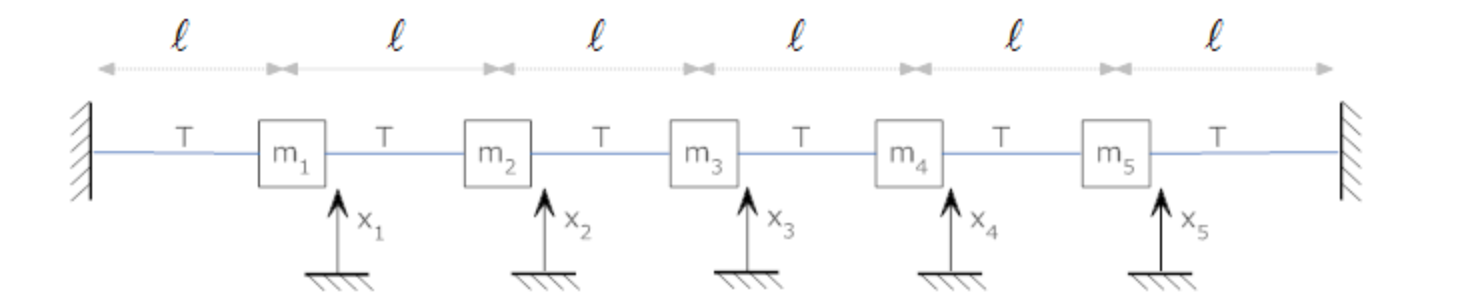
\includegraphics[scale=0.2]{11.png}
    \caption{微振动系统示意图}
\end{figure} 

如图,\ \ 5个质量均为m的物块在均匀张力
1$T_n$下的弦上物块进行距离$l$的等距分布。每个物体$m_i$
均只可以在竖直方向进行微振动,并且对每个物
块
都有一个竖直方向的位移$ x _i$.
\subsubsection{对于研究对象的实际分析}

显然的,本系统符合微振动的定义,故而我们可以通过
之前提到的分析方法进行实际分析.

再次陈列一下基本步骤


\textbf{(\romannumeral1)写出体系的拉格朗日量}

\textbf{(\romannumeral2)对体系能量进行简谐近似}

\textbf{(\romannumeral3)将近似之后的拉格朗日量代入拉格朗日方程}

\textbf{(\romannumeral4)用傅里叶变换或者二次型对角化方法脱耦}

\textbf{(\romannumeral5)利用脱耦之后的拉格朗日方程,求出本征频率与简正模}

\textbf{(\romannumeral6)结合给出的初始条件,计算出每个简正模式的贡献,得出运动方程}

\vspace{5mm}
对于本题具体情况,我们对于基本步骤进行了一些简化,具体步骤如下

\vspace{5mm}
\textbf{(\romannumeral1)写出体系的拉格朗日量}
\vspace{5mm}

首先进行系统力学分析,不妨对于下图这种情况进行分析
\begin{figure}[h]
	
    \centering
    \vspace{4mm}
    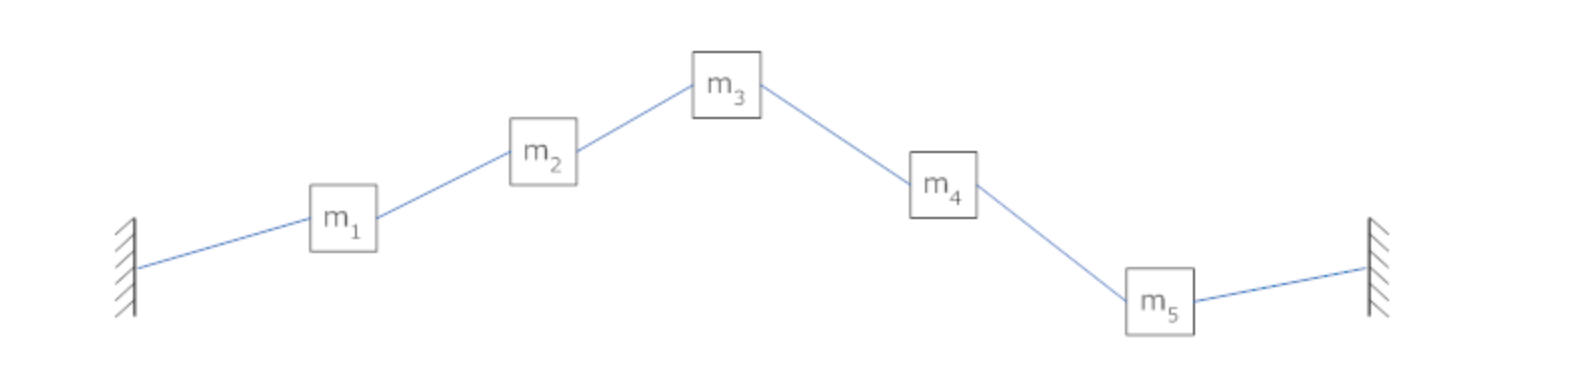
\includegraphics[scale=0.2]{22.png}
    \caption{微振动系统状态示意图}
\end{figure} 



\begin{figure}[h]
	
    \centering
    \vspace{4mm}
    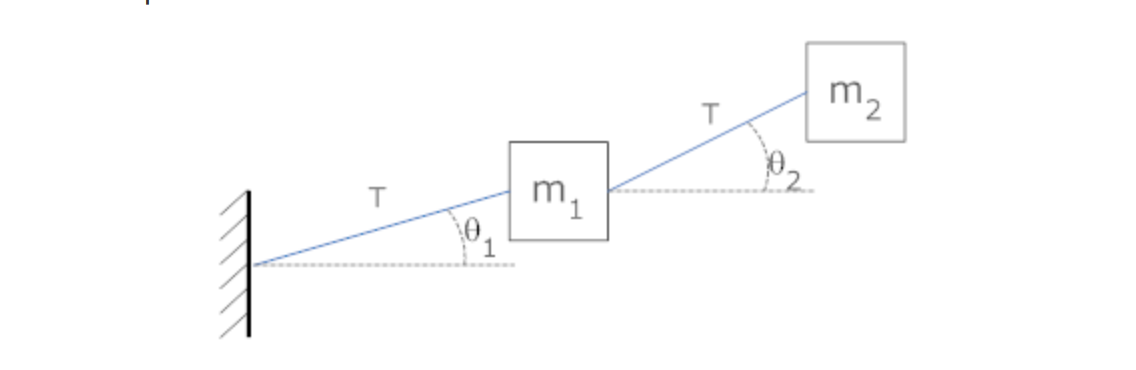
\includegraphics[scale=0.2]{33.png}
    \caption{微振动系统}
\end{figure} 

由图2,3我们可以作出受力分析如下

\begin{figure}[h]
	
    \centering
    \vspace{4mm}
    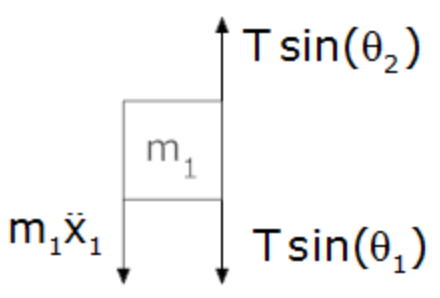
\includegraphics[scale=0.2]{44.png}
    \caption{受力分析图}
\end{figure} 

由此我们可以得到系统中每个物体的动能和势能

\begin{equation}
    T = \sum_{i=0}^5\frac{1}{2}m_i\dot{x}_i
\end{equation}
\begin{equation}
    V = \sum_{i=0}^5T_n\left(-sin\theta_{l_i}x_i+sin\theta_{r_i}x_i\right.)
\end{equation}

由于微振动,其中
\begin{equation}
    sin\theta_{l_i}=\frac{xi}{l},\quad sin\theta_{r_i}=\frac{\Delta x_i}{l}
\end{equation}

可以写出拉氏量为:
\begin{equation}
    \mathscr{L}=\sum_{i=0}^5\frac{1}{2}m_i\dot{x}_i+V(i)
\end{equation}

其中$V$的大小与物块受力有关,其中受力与物块位置有关(受力数目)

\vspace{5mm}
\textbf{(\romannumeral2)将近似之后的拉格朗日量代入拉格朗日方程}

\vspace{5mm}代入

\begin{equation}
    \frac{d}{dt}\frac{\partial\mathscr{L}}{\partial \dot x_i}
    +\frac{\partial\mathscr{L}}{\partial x_i}
    = 0
\end{equation}

故拉格朗日方程为

\begin{equation}
    \left\{
    \begin{aligned}[l]
    &\ddot{x}_{1}=&-&2 \frac{T_n}{m} x_{1}&+&\frac{T_n}{m} x_{2} \\
    &\ddot{x}_{2}=\frac{T_n}{m} x_1&-&2 \frac{T_n}{m} x_{2}&+&\frac{T_n}{m} x_3 \\
    &\ddot{x}_{3}=\frac{T_n}{m} x_2&-&2 \frac{T_n}{m} x_{3}&+&\frac{T_n}{m} x_{4} \\
    &\ddot{x}_{4}=\frac{T_n}{m} x_{3}&-&2 \frac{T_n}{m} x_{4}&+&\frac{T_n}{m} x_{5} \\
    &\ddot{x}_{5}=\frac{T_n}{m} x_{4}&-&2 \frac{T_n}{m} x_{5}
    \end{aligned}\right.
\end{equation}

可以写为矩阵形式为


\begin{equation}
    \ddot{\boldsymbol{x}}=\boldsymbol{A'} \cdot \boldsymbol{x}=\frac{T_n}{m}\boldsymbol{A} \cdot \boldsymbol{x}=\frac{T_n}{m}\left
    [\begin{matrix}\vspace{-1.5ex}
    -2 & 1 & 0 & 0 & 0 \\\vspace{-1.5ex} 
    1 & -2 & 1 & 0 & 0 \\\vspace{-1.5ex} 
    0 & 1 & -2 & 1 & 0 \\\vspace{-1.5ex} 
    0 & 0 & 1 & -2 & 1 \\\vspace{-1.5ex} 
    0 & 0 & 0 & 1 & -2\vspace{2.5ex} 
    \end{matrix}\right] \boldsymbol{x}
    \end{equation}

\vspace{5mm}
    \textbf{(\romannumeral3)利用脱耦之后的拉格朗日方程,求出本征频率与简正模}
    \vspace{5mm}

    对矩阵 $\boldsymbol A'$ 求解本征值与本征矢即对矩阵$\boldsymbol A$求本征值与本征矢;
    本征值即对应的本征频率的平方,本征矢即本征频率对应的振动矢量。利用后续介绍的数值计算方法求解
    本征值与本征矢即可。




\vspace{5mm}
\textbf{(\romannumeral4)结合给出的初始条件,计算出每个简正模式的贡献,得出运动方程}
\vspace{5mm}

上一步我们可以得到\{$\omega_1,\omega_2,\omega_3,\omega_4,\omega_5$\}五个本征频率和\{$\boldsymbol{v_1,v_2,v_3,v_4,v_5}$\}五个本征矢,不妨令$\boldsymbol {V}=[\boldsymbol{v_1,v_2,v_3,v_4,v_5}]$
不难得到
\begin{equation}
    \boldsymbol {V} \boldsymbol\gamma_1 = \boldsymbol x(0)
\end{equation}
\begin{equation}
    \boldsymbol {V}\  \boldsymbol {Diag}(\omega_1,\omega_2,\omega_3,\omega_4,\omega_5)\boldsymbol\gamma_2 = \boldsymbol{\dot x}(0) 
\end{equation}
其中,在一般情况下公式(13)等价于
\begin{equation}
    \boldsymbol {Diag}(\omega_1,\omega_2,\omega_3,\omega_4,\omega_5)\boldsymbol\gamma_2 = \boldsymbol {V}^{-1} \boldsymbol{\dot x}(0) 
\end{equation}
由此可以得到$\boldsymbol{\gamma_1,\gamma_2}$两个决定简正模式贡献的常数向量,由此结合公式(22)
$$
    \bm x(t)=\bm{\gamma_{1}}\ cos(\omega_it)+\bm{\gamma_{2}}\ sin(\omega_it
$$
即可得出各个物体的运动方程。

\newpage
\section{数值计算}
{
    理论分析过程已经得出了较为清晰的分析思路,并且得到了拉格朗日方程
    下面来讨论从
    数值计算角度解决问题。


}
\subsection{计算思路}
{
    首先,根据公式(29)
    $$
        \ddot{\boldsymbol{x}}=\boldsymbol{A'} \cdot \boldsymbol{x}=\frac{T_n}{m}\boldsymbol{A} \cdot \boldsymbol{x}=\frac{T_n}{m}\left
        [\begin{matrix}\vspace{-1.5ex}
        -2 & 1 & 0 & 0 & 0 \\\vspace{-1.5ex} 
        1 & -2 & 1 & 0 & 0 \\\vspace{-1.5ex} 
        0 & 1 & -2 & 1 & 0 \\\vspace{-1.5ex} 
        0 & 0 & 1 & -2 & 1 \\\vspace{-1.5ex} 
        0 & 0 & 0 & 1 & -2\vspace{2.5ex} 
        \end{matrix}\right] \boldsymbol{x}
    $$
以及前置理论我们得知,求解出矩阵$\boldsymbol A$
的本征值和本征向量稍作变化便可得到本征频率与本征矢,
带入初值求解
$$
    \boldsymbol {V} \boldsymbol\gamma_1 = \boldsymbol x(0)
$$$$
    \boldsymbol {V}\  \boldsymbol{Diag}(\omega_1,\omega_2,\omega_3,\omega_4,\omega_5)\boldsymbol\gamma_2 = \boldsymbol{\dot x}(0) 
$$
两个方程即可得到各个振动模式的贡献,得出数值解。

因此计算思路如下:


{\hspace{8mm}\textbf{(\romannumeral1)估算出本征值的范围选取合适的求解方法}

\hspace{8mm}\textbf{(\romannumeral2)求出本征值}

\hspace{8mm}\textbf{(\romannumeral3)用合适方法求出本征向量}

\hspace{8mm}\textbf{(\romannumeral4)用合适方法求出振动模式的贡献}

\hspace{8mm}\textbf{(\romannumeral5)绘制出振动图像}}

其中,最重要的是计算过程中的\textbf{精度控制}以及\textbf{方法选取},
两个重点会互相影响,在后续讨论中会有所说明。


}

\subsection{计算实现}
\subsubsection{$\mathbf {Gershgorin}$圆盘定理判断本征频率的范围}
{
    首先,我们需要得到本征值的大致范围,(至少精确到本征值数量和数量级)以此选择大概的本征值
    计算方法(这一步骤是常规解析求解中或许是不必要的,但是我认为
    在数值计算中对于算法的选取有影响意义)。其中$ {Gershgorin}$圆盘定理是一个可行的方法。
    
    $ {Gershgorin}${圆盘定理}有下述两个定理组成
    \vspace{2mm}

    \textbf{定理\ 2}(Gershgorin
    圆盘第一定理):
    
    \emph{设}$\boldsymbol {A}$\emph{是n
    阶矩阵,}$\ \boldsymbol A={a_{ij}}_{(n \times n)},\ ${\emph 则
    $\boldsymbol A$   \emph{的本征值在复平面上下列圆盘(Gershgorin 圆盘)中:
    }
    $$
    \left|z-a_{i i}\right| \leq R_{i}, i=1,2, \cdots, n
    $$
    \emph{其中} $R_{i}$ \emph 为 $A$ \emph{的第{} $i$
    行元素去掉 $a_{i i}$ 后的模之和, 即
    $$R_{i}=\sum_{j \neq i}^{n}\left|a_{i j}\right|=\left|a_{i 1}\right|+\cdots+\left|a_{i, i-1}\right|+\left|a_{i, i+1}\right|+\left|a_{i n}\right| \quad$$ 
    }
    \vspace{-6mm}

    \textbf{定理\ 3}(Gerschgorin圆盘第二定理):
    
    \emph{设矩阵 $A=\left(a_{i j}\right)_{n \times n}$ 的 $n$ 个Gershgorin
    圆盘分成若干个连通区 域, 若其中一个连通区域含有 $k$ 个Gershgorin
    圆盘, 则有且只有 $k$ 个本征值落在这个连通区域内(若两 个Gershgorin
    圆盘重合, 需计重数; 又若本征值为重根, 也计重数).
    }

    
    按照\textbf{定理2},利用python画图功能\footnote{Gershgorin圆盘图片绘制程序实现见附录}
    我们可以作出如下图片:
    \begin{figure}[h]
	
        \centering
        \vspace{4mm}
        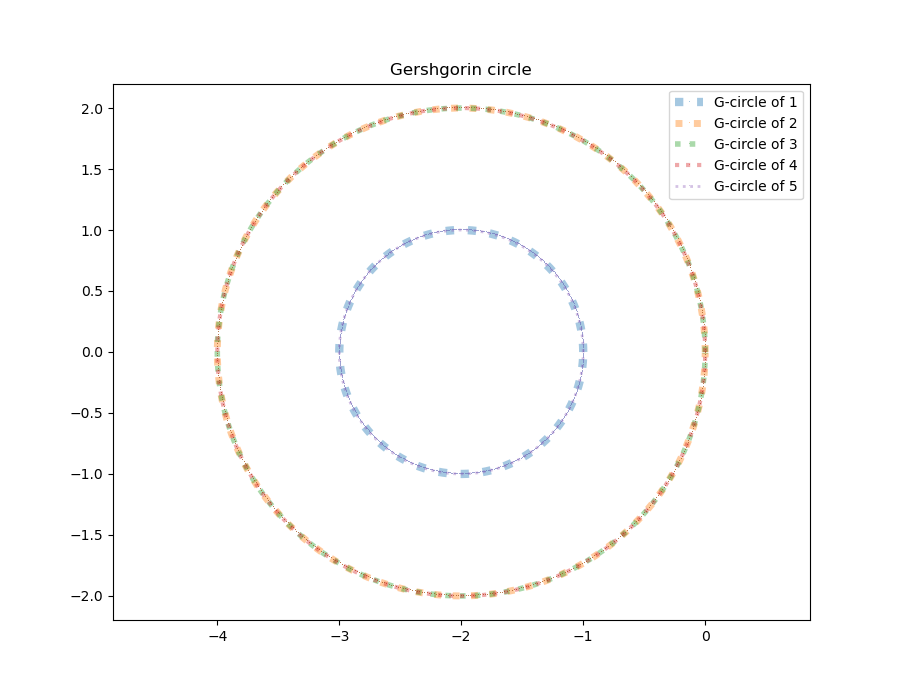
\includegraphics[scale=0.55]{Gershgorin_circle.png}
        \caption{Gerschgorin圆盘图}
    \end{figure} 

由于上述定理,结合
图 5,以及矩阵$\boldsymbol{A}$严格对角占优
,我们可以得到以下几点结论:

$\bullet$矩阵$\boldsymbol{A}$为可逆矩阵

$\bullet$矩阵$\boldsymbol{A}$本征值一定都为负数

$\bullet$矩阵$\boldsymbol{A}$所有本征值一定都介于[-4,0]之间

由于本题矩阵的对称性极强,可以证明\cite{a}\textbf{以上结论对于自由度更大的时依然成立}。

不难看出本征值的模应该不小于0.1,因此所有本征值
都与矩阵各非零元数量级大致相同,不用过分担心由于
算法造成的误差,故而可以适用绝大多数算法(不过原点平移法
或许会由于本征值过于接近而出现问题,故本题并没有尝试)。

(本课题中矩阵过于简单,Gershgorin圆盘法作用未能完全显现)

    


    % {    \begin{flushright}
    % \scriptsize\emph{运行环境\\$Ubuntu 9.3.0-17\ Ubuntu1~20.04LTS$}\\
    % \scriptsize\emph{$Python 3.8.8$\ \ $Anaconda 4.10.3\ \  AMD-4800u$}
        
    % \end{flushright}
    % \inputpython{Gerschgorin-plt.py}{1}{35}

    % }
\subsubsection{$Jacobi$ 方法求解本征频率与本征矢}

理论分析得到,本征频率的平方为本征值,故而
本步骤目的变为
本征值与本征向量,对矩阵进行对角化可以同时得到上述
预期结果。
考虑到矩阵可逆以及为实对称矩阵,本次
采用$Jacobi$方法,用$Givens$
旋转矩阵进行正交对角化。

从结果出发,只要可以成功得到
$$\boldsymbol{A}=\boldsymbol P^T \boldsymbol B \boldsymbol P$$
这个形式,其中$\boldsymbol B$为对角矩阵
,$\boldsymbol P$为正交矩阵,我们就可以得到矩阵$\boldsymbol A$
的本征值与对应本征向量,其中本征值为$\boldsymbol B$
的对角元,本征向量为$\boldsymbol P$矩阵对应的列向量。

因此,我们需要找到合适的矩阵$\boldsymbol P$
以及对应矩阵$\boldsymbol B$使其满足上述条件,
成功将$\boldsymbol A$对角化为$\boldsymbol B$
。对于本题来讲,我们可以认为非对角元素之和小于$10^{-15}$
即为成功对角化。

$\bullet Jacobi$方法

我们之前说到我们需要把$\boldsymbol A$
对角化,他的目的是通过一次次的合适的正交相似变换
进行形如
$$\boldsymbol A_{i+1}=\boldsymbol 
Q^T \boldsymbol {A}_i \boldsymbol Q$$
的迭代,将A转化为
$$\boldsymbol Q_n^T \dots\boldsymbol Q_2^T \boldsymbol Q_1^T 
\boldsymbol {A}_n 
\boldsymbol Q_1\boldsymbol Q_2\dots \boldsymbol Q_n$$
的形式,显然的,如果矩阵$\boldsymbol Q$选取合适
可以达到对角化的作用。一般$Jacobi$都和误差控制
结合使用,达到需要精度之后跳出迭代即可。

$\bullet Givens$旋转矩阵

$Givens$旋转矩阵表示为如下形式的矩阵
$$
\boldsymbol G(i, j, \theta)=\left[\begin{array}{ccccccc}
1 & \cdots & 0 & \cdots & 0 & \cdots & 0 \\
\vdots & \ddots & \vdots & & \vdots & & \vdots \\
0 & \cdots & c & \cdots & s & \cdots & 0 \\
\vdots & & \vdots & \ddots & \vdots & & \vdots \\
0 & \cdots & -s & \cdots & c & \cdots & 0 \\
\vdots & & \vdots & & \vdots & \ddots & \vdots \\
0 & \cdots & 0 & \cdots & 0 & \cdots & 1
\end{array}\right]
$$
这里的 $c=\cos (\theta)$ 和 $s=\sin (\theta)$ 出现在第 $i$ 行和第 $j$ 行与第 $i$ 列和第 $j$ 列的交叉点上。就是说, $Givens$旋转矩阵的所有非零元定义如下: :
$$
    \left\{
        \begin{aligned}
            g_{k k} &=1 \quad \text ({ for \ \ } k \neq i, j) \\
            g_{i i} &=c \\
            g_{j j} &=c \\
            g_{i j} &=s \\
            g_{j i} &=-s
        \end{aligned}
        \right.
$$
$\boldsymbol G(i, j, \theta) \boldsymbol x$  表示向量 $\boldsymbol{x}$ 在 $(i, j)$ 平面中的逆时针旋转 $\theta$ 弧度。
Givens 旋转在数值线性代数中主要的用途是在向量或矩阵中介入零。
这个本步的目的不谋而合。同时他还有便于并行计算和对于稀疏矩阵
支持较好两个优点,对于本题的高自由度情况有较大用处。

结合上述介绍,我们不难想到用$Givens$矩阵来进行$Jacobi$
方法进行对角化,显然的旋转矩阵的正交性完美满足要求,
接下来的问题就只需要生成矩阵并通过迭代达成
$$\boldsymbol {A} _n=\boldsymbol G_n^T \dots\boldsymbol G_2^T \boldsymbol G_1^T 
\boldsymbol {A} 
\boldsymbol G_1\boldsymbol G_2\dots \boldsymbol G_n$$
从而得到正交化之后的$\boldsymbol A_n$.而这一步
通过对于A矩阵进行不断的左乘右乘即可实现。

同时,由于$Givens$矩阵十分稀疏,我们不妨将其展开
得到如下公式
$$
    \left\{\begin{array}{l}
    	b_{i p}=b_{p i}=a_{p i} \cos \theta-a_{q i} \sin \theta, \quad i \neq p, q \\
    	b_{i q}=b_{q i}=a_{p i} \sin \theta+a_{q i} \cos \theta, \quad i \neq p, q \\
    	b_{p p}=a_{p p} \cos ^{2} \theta+a_{q q} \sin ^{2} \theta-a_{p q} \sin 2 \theta \\
    	b_{q q}=a_{p p} \sin ^{2} \theta+a_{q q} \cos ^{2} \theta+a_{p q} \sin 2 \theta \\
    	b_{p q}=b_{q p}=a_{p q} \cos 2 \theta+\frac{a_{p p}-a_{q q}}{2} \sin 2 \theta
    \end{array}\right.
    $$

通过这项变换,进行一次循环即可得到
$$\boldsymbol A_{(i)}=\boldsymbol G_{(i)}^T 
\boldsymbol {A}
\boldsymbol G_{(i)}$$
的结果。不难注意到时间复杂度从
$O(n^3)$变成了$O(n)$,在矩阵维数较大的时候
可以极大加快运算。

上式中的第二个等式以及模态矩阵和本征向量的关系可以得出一个对角矩阵,
本步骤用到了$Jacobi$,矩阵乘法,矩阵转置三个函数\footnote{完整程序实现见附录},上述操作可以在$Jacobi$
函数中把两次矩阵乘法加上一次矩阵转置化为一体,达到
加速效果。

最终得到的对角矩阵的对角元便是本征频率的绝对值,右侧矩阵的列向量便是
本征矢。


    {    \begin{flushright}
    \scriptsize\emph{运行环境\\$Ubuntu 9.3.0-17\ Ubuntu1~20.04LTS$}\\
    \scriptsize\emph{$Python 3.8.8$\ \ $Anaconda 4.10.3\ \  AMD-4800u$}
        
    \end{flushright}
    \inputpython{5_pic.py}{3}{3}
    \inputpython{5_pic.py}{14}{73}
    \inputpython{5_pic.py}{74}{81}
    \inputpython{5_pic.py}{82}{88}
    }
\subsubsection{初值讨论}

\par 经过上述处理后,我们可以得到$$\boldsymbol {A}_{(n)}=\boldsymbol G_n^T \dots\boldsymbol G_2^T \boldsymbol G_1^T 
\boldsymbol {A}
\boldsymbol G_1\boldsymbol G_2\dots \boldsymbol G_n$$的对角化形式。
其中$\boldsymbol A_n$为
对角矩阵,对角值为本征值。左右都为本征向量组成的矩阵。

\par 代入之前得到的解$$
\bm x(t)=\bm{\gamma_{1}}\ cos(\omega_it)+\bm{\gamma_{2}}\ sin(\omega_it)
$$
带入之前的拉格朗日方程
$$
\sum_jm_{ij}\ddot x_j + \sum_k k_{ij} x_j = 0
$$
并且结合$$
\boldsymbol {V} \boldsymbol\gamma_1 = \boldsymbol x(0)
$$$$
\boldsymbol {V}\  \boldsymbol {Diag}(\omega_1,\omega_2,\omega_3,\omega_4,\omega_5)\boldsymbol\gamma_2 = \boldsymbol{\dot x}(0) 
$$
给出$2s=10$个初值,我们就可以得到$\bm{\gamma_{1}},\bm{\gamma_{2}}$
的解,从而得到振动方程。求解过程在本部分将采用直接用$\boldsymbol V^T = \boldsymbol V^-1$来求解
$\boldsymbol\gamma_1 ,\boldsymbol\gamma_2$.
\footnote{程序实现见附录}


    
\subsubsection{运动状态与图像给出}
{
带入初值得到最终的运动方程,我们便可以进行运动图像的绘制
,一般的,我们可以分别得到五个不同的运动图像,绘制在
同一张图像我们可以得到并比较其运动状态。注意选取合适的
且确定的横纵坐标范围,以得到较为稳定的图像便于比较
\footnote{程序实现见附录}。
}



\subsection{计算结果}
{
    


根据上述方法计算矩阵的本征值与本征向量我们可以得到如下结果

% Please add the following required packages to your document preamble:
% \usepackage{booktabs}
\begin{table}[h]
    \centering
    \caption{5自由度系统本征值}
    \begin{tabular}{@{}p{2cm}<{\centering}p{2cm}<{\centering}p{2cm}<{\centering}p{2cm}<{\centering}p{2cm}<{\centering}@{}}
    \toprule
    \multicolumn{5}{c}{本征值}                  \\ \midrule
    -3 & -1 & -3.73205081 & -0.26794919 & -2 \\ \bottomrule
    \end{tabular}
    \end{table}
% Please add the following required packages to your document preamble:
% \usepackage{booktabs}
\begin{table}[h]
    \caption{5自由度系统本征矢}
    \centering
    \begin{tabular}{@{}p{2cm}<{\centering}p{2cm}<{\centering}p{2cm}<{\centering}p{2cm}<{\centering}p{2cm}<{\centering}@{}}
    \toprule
    \multicolumn{5}{c}{本征向量}                              \\ \midrule
    {}0.5 & 0.5  & 0.28867513 & 0.28867513 & 0.57735027  \\
    -0.5   & 0.5  & -0.5       & 0.5        & 0.          \\ 
    -0.    & 0.   & 0.57735027 & 0.57735027 & -0.57735027 \\
    0.5    & -0.5 & -0.5       & 0.5        & 0.          \\
    -0.5   & -0.5 & 0.28867513 & 0.28867513 & 0.57735027  \\\bottomrule
    \end{tabular}
    \end{table}

    不妨取初值$\boldsymbol{x_0}=[1,0,0,0,0]^T,
    \boldsymbol{\dot x_0}=[0,0,0,0,0]^T
    $(与微振动系统来源的默认值一样),我们可以得到
    $\boldsymbol\gamma_1,\ \omega\boldsymbol\gamma_2 $
% Please add the following required packages to your document preamble:
% \usepackage{booktabs}
\begin{table}[h]
    \centering
    \caption{5自由度系统在初值1下$\gamma_1,\omega\gamma_2值$}

    \begin{tabular}{@{}p{1cm}<{\centering}p{2cm}<{\centering}p{2cm}<{\centering}p{2cm}<{\centering}p{2cm}<{\centering}p{2cm}<{\centering}@{}}
    \toprule
    $\gamma_1$       & 0.5 & 0.5 & 0.28867513 & 0.28867513 & 0.57735027 \\ \midrule
    $\omega\gamma_2$ & 0   & 0   & 0          & 0          & 0          \\ \bottomrule
    \end{tabular}
    \end{table}
    
    代入$\bm x(t)=\bm{\gamma_{1}}\ cos(\omega_it)+\bm{\gamma_{2}}\ sin(\omega_it)
    $可以作出如下图像。
    
    \begin{figure}[!ht]
        
        \centering
        \vspace{2mm}
        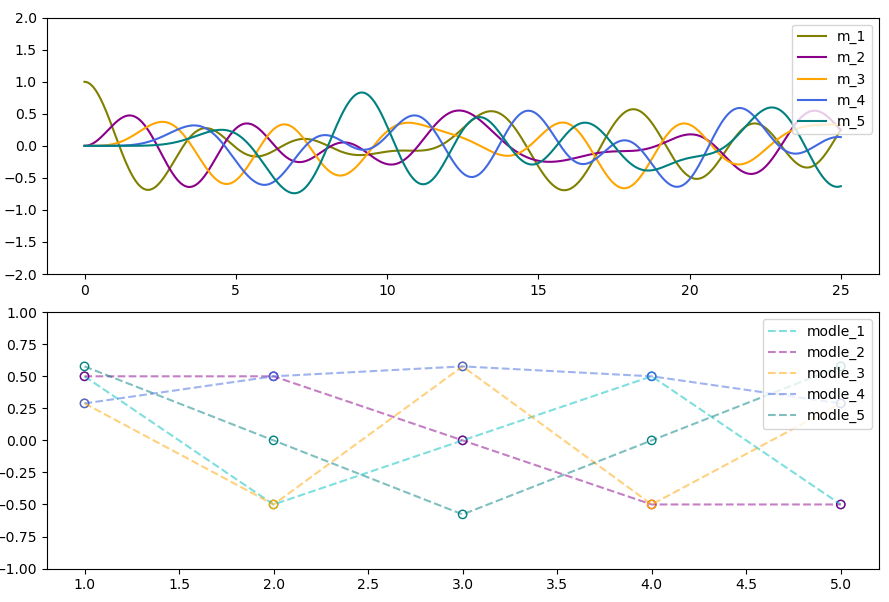
\includegraphics[scale=0.6]{pic5_png.png}
        \caption{在初值1状态下的振动图以及本征向量图 }
    \end{figure} 

    至此,我们已经完美完成了网站上项目的复现,
    并且进行了速度初值的计算以及参与结果。


} 
\subsection{结果与讨论}
根据以上计算,我们可以得到五自由度的微振动系统的
数值运动解。
\subsubsection{结果陈列}
\vspace{5mm}
\textbf{初值2}

$\bullet\quad\boldsymbol{x_0}=[1,0,0,0,1]^T,
\boldsymbol{\dot x_0}=[1,0,1,0,1]^T
$

\begin{table}[h]
    \centering
    \caption{5自由度系统在初值2下$\gamma_1,\omega\gamma_2值$}

    \begin{tabular}{@{}p{1cm}<{\centering}p{2cm}<{\centering}p{2cm}<{\centering}p{2cm}<{\centering}p{2cm}<{\centering}p{2cm}<{\centering}@{}}
    \toprule
    $\gamma_1$       & 0 & 0 & 0.57735 & 0.57735 & 1.1547 \\ \midrule
    $\omega\gamma_2$ & 0   & 0   & 1.1547         &    1.1547       & 0.57735        \\ \bottomrule
    \end{tabular}
    \end{table}
    \vspace{2mm}
    \textbf{初值3}

    $\bullet\quad\boldsymbol{x_0}=[-1,1,0,-1,1]^T,
    \boldsymbol{\dot x_0}=[1,-1,0,1,-1]^T
    $

    \begin{table}[h]
        \caption{5自由度系统在初值3下$\gamma_1,\omega\gamma_2值$}
        \centering
        \begin{tabular}{@{}p{1cm}<{\centering}p{2cm}<{\centering}p{2cm}<{\centering}p{2cm}<{\centering}p{2cm}<{\centering}p{2cm}<{\centering}@{}}
        \toprule
        $\gamma_1$       & 2 & 0 & 0 & 0 & 0 \\ \midrule
        $\omega\gamma_2$ & 2   & 0   & 0        &    0       & 0     \\ \bottomrule
        \end{tabular}
        \end{table}


    \begin{figure}[h]
        
        \centering
        \vspace{2mm}
        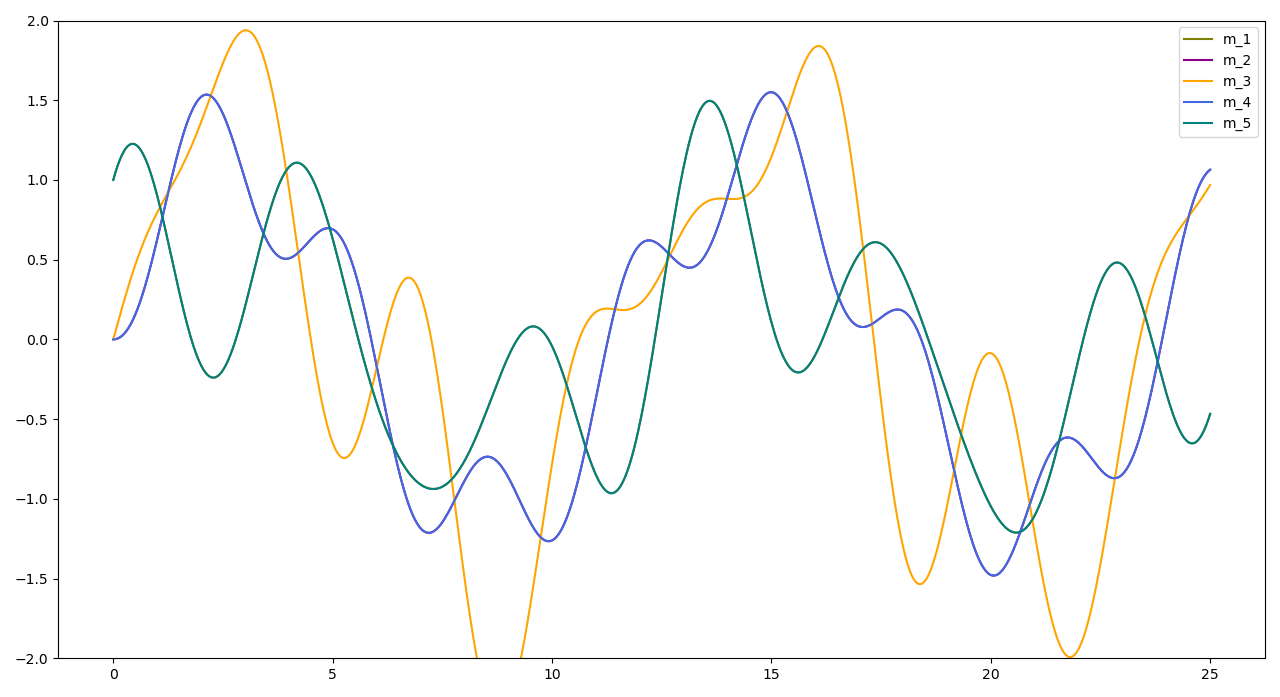
\includegraphics[scale=0.4]{1,0,1,0,1.png}
        \caption{在初值2状态下的振动图 }
    \end{figure} 

    \begin{figure}[H]
        
        \centering
        \vspace{2mm}
        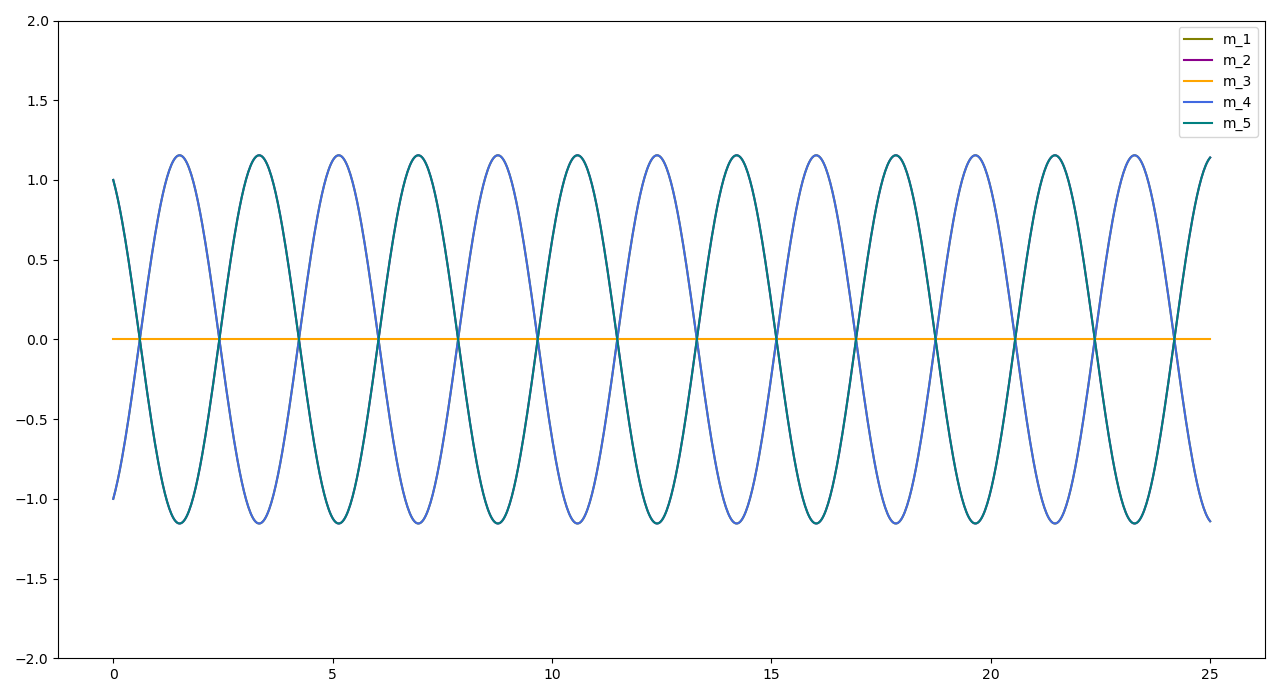
\includegraphics[scale=0.4]{1,-1,0,1,-1.png}
        \caption{在初值3状态下的振动图 }
    \end{figure} 
    

\subsubsection{对称性讨论}

之前的初值选取是有技巧的,我们可以看出系统振动有极高的
对称性
,这是因为我们选取的初值与模式形状的对称性匹配。
例如,初值 3${x_0}=[-1,1,0,-1,1]^T,
\boldsymbol{\dot x_0}=[1,-1,0,1,-1]^T
$的对称性
与且仅与$modle_1$完美匹配,故其有且仅有唯一激发的$\omega=1.73205081$
.类似细节不多赘述,由此我们得到激发特定频率的方式。

同时,我们可以证明初速度的对称性和初位移的对称性是独立的
,也就是说改变速度不影响频率。
\subsubsection{question:如何激活特定频率}

不难证明,

由上,我们知道了对称性的初值可以激发有相同对称性的频率,
一般的,如果初值的对称性是振动$modle$对称性的耦合
我们也可以得到具有耦合关系的频率。

因此我们有了激活特定频率的一般性思想:可以通过初值的
选取来激活特定频率。
\subsection{多自由度分析}
\subsubsection{多自由度情况矩阵生成}
显然的,根据上述理论得到该矩阵是解题的首要关键。

矩阵形如

$$
\left[\begin{array}{ccccc}
-2 & 1 &   & \\
1 & -2 & \ddots & & \\
& \ddots & \ddots  & \ddots & \\
&   & \ddots & -2 & 1 \\
&   & & 1 & -2
\end{array}\right]
$$
用双重循环即可得到该矩阵,具体计算方式不再赘述。

\subsubsection{多自由度本征求解}

函数计算思路大体不变,不过之前时间复杂度的考量有了存在意义。

不妨考虑$s=1000$的情况,即矩阵为1000维。
我们可以得到1000个本征值。
按照自由度展开做图可得
\begin{figure}[H]
        
    \centering
    \vspace{2mm}
    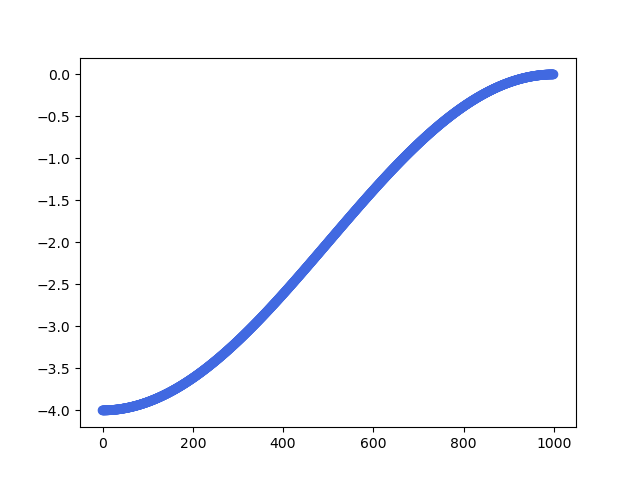
\includegraphics[scale=0.45]{v-1000.png}
    \caption{本征值-自由度图像 }
\end{figure} 
不难想到,在自由度足够的情况下,本征值将会
遍历$Gerschgorin\ Circle$的实数区,即所有可能的
本征值位置。

按照同样的方法,我们可以得到本征解并且绘出振动图像
节约时间,取$s=100$,初值为初值1,我们可以得到如下图像
\begin{figure}[H]
        
    \centering
    \vspace{2mm}
    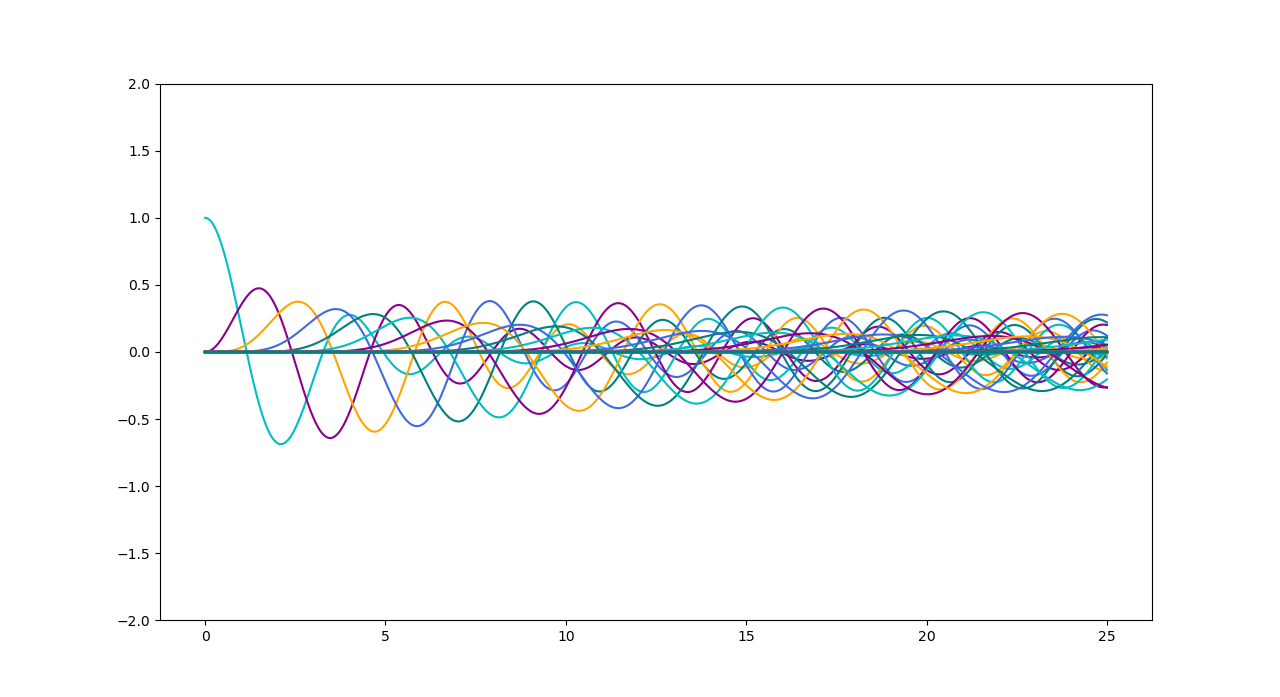
\includegraphics[scale=0.4]{100_pic.png}
    \caption{振动-时间图像 }
\end{figure} 

或许这张图过于杂乱不清晰,通过下面这张图可以看出
可以看出波传播的趋势——我们得到了标准的驻波图像(美观起见
s分别取为2000和10000,为了得到稳定图像,t取$t= 2000000$算法优化不够,调用了$numpy$的函数).
(留意其横纵坐标)

\newpage

自由度为2000的微振动系统在
t时刻的波形如下

\begin{figure}[H]
        
    \centering
    \vspace{2mm}
    \includegraphics[scale=0.4]{200000_2000.png}
    \caption{t=2000000,s=2000的波形图 }
\end{figure} 


\vspace{7mm}
自由度为10000的微振动系统在
t时刻的波形如下

\begin{figure}[H]
        
    \centering
    \vspace{2mm}
    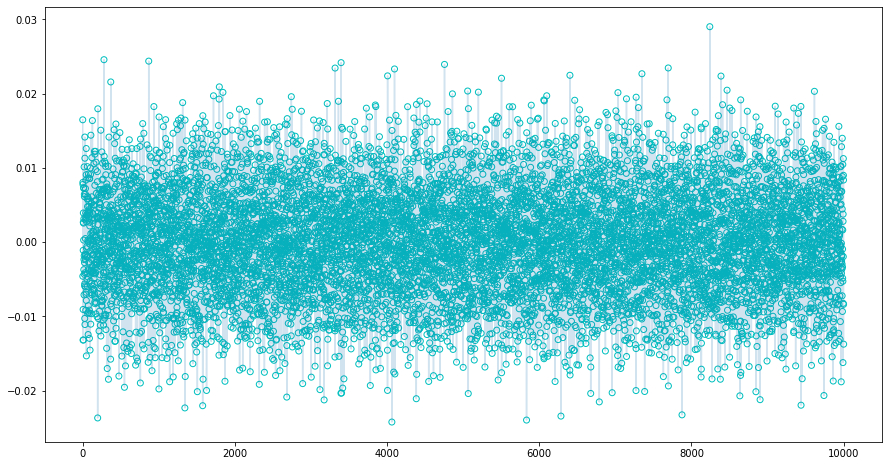
\includegraphics[scale=0.4]{200000_10000.png}
    \caption{t=2000000,s=10000的波形图 }


\end{figure} 

\vspace{7mm}
我们可以看出,此时振动已经形成了驻波形式,并且能量
分配的较为均匀,不过只有t=2000000的波形图不够直观
我们不妨作出波形图的演化图像


\vspace{5mm}
P.S.演化图像为动态图,建议使用Adobe Acrobat dc,Okular等软件打开本文档

\newpage

振动从左端传递到右端过程的图像如下

\begin{figure}[H]
\centering
\vspace{-3mm}
    \animategraphics[width=6in,height=3.5in,autoplay,loop]{30}{A}{1}{200}
    \vspace{-8mm}
    \caption{s=2000,t=[0-1999]时间间隔取10,FPS=30的波形演化图}
\end{figure} 

驻波形成图像见下(速度为上图的2.5倍)

\begin{figure}[H]
\centering
\vspace{-3mm}
     \animategraphics[width=6in,height=3.5in,autoplay,loop]{30}{B}{1}{321}
\vspace{-8mm}
\caption{s=2000,t=[2000-10001]时间间隔取25,FPS=30的波形演化图}
\end{figure} 

其物理意义将于后续部分再行探究。
{
    
   
        
}

\newpage
\section{问题分析与探讨}
{
    在进行多自由度微振动的本正频率问题的数值计算时,
    我们主要遇到了如下问题

    $\cdot$本征向量的求出

    $\cdot$精度问题

    $\cdot$初值计算
    
    $\cdot$时间复杂度过高

    $\cdot$物理意义不明确
    
    下面对各个问题的进行讨论。
}
\subsection{问题概述与解决}
\subsubsection{本征向量的求出}
在求出本征向量的过程中,最显而易见的便是直接用$Givens$
矩阵的连乘,不过我们在讨论过程中肯定会有疑问:用迭代法
求解或者矩阵分解求解可以吗?

矩阵分解法显然是可以的,不过普遍的分解法时间复杂度过高
,而对称QR分解虽然时间复杂度降低到了$O_{(n)}$\cite{a},可是用QR求解
方程需要循环次数过高,故而也不予以考虑。

至于迭代方法,我们常用的雅可比法,高斯-赛德尔迭代,以及松弛迭代法
都有一个通用的收敛条件:谱半径大于1,目前暂且没有查到
或者自己想到合适的
优化算法,因此没有考虑。

故而,目前采用的还是连乘$Givens$矩阵,时间还在可接受范围内。
同时由于Givens矩阵十分稀疏,因此如果展开用元素写出还有更大
优化空间。最终可以得到一个时间复杂度为$O_{(n)}$的算法
,不过在python上的实现仍距有距$numpy$有较大距离。
\subsubsection{精度问题}
本次课题主要用的是$Jacobi$迭代求解本征向量与本征值,
因此我们需要考虑何时退出迭代。

同时在求$sin\theta$等三角函数时,我使用了
python中numpy库里面的三角函数包,经尝试可以有效增加精度
。

显然的,迭代次数会随着矩阵维数增加而增加,我们不妨设定
非对角元绝对值之和$<10^{-15}$即为成功对角化,
最终误差期望应该在$10^{-15}$左右。

\subsubsection{初值计算}
初值计算等价与解线性方程组,
线性方程组的解法多样回归到了类似之4.1.1的
问题。同样的,控制谱半和优化算法都是较难的工作
同时在$s<100$时,整体程序运行时间均不超过20s,因此
没有作出计算方法的创新。


\subsubsection{时间复杂度过高}

时间复杂度过高主要是由于循环过多。
例如,矩阵乘法的三重循环,寻找最佳旋转角
的双重循环,矩阵赋值的双重循环等$\dots\dots$
(只考虑考虑双重以上循环)

对于矩阵乘法,我们应该在可以简化的地方(例如
$Givens$矩阵的矩阵运算展开,对元素求解
。同样的寻找最佳旋转角也应该利用的
对称性
进行对角线搜索,矩阵赋值多用深度复制(copy.deepcopy())
,等,对于时间复杂度已有较好优化,当然还有更多想法由于能力不足
未能实现。

\subsubsection{物理意义不明确}

最开始我不是很了解弹力大小不变的微振动物理意义,
直到接触到弦震动方程想到了增加自由度来逼近。

此外,查阅文献发现更符合的情况是边界条件为
质量无穷大原子的一维原子链,下一部分将会进行解析求解对比。

    }
\subsection{解析求解对比}
{
    固定边界条件下的一维原子链的集体振动和本题
    描述的是十分相似,故而进行解析讨论。

    一纬原子链是固体物理中的常用模型,其考虑了原子之间的
    作用里考虑在有初值条件下的运动情况,本题的实质是固定边界条件下的一维单原子链,下面进行讨论。

    在简谐近似下,一维原子链可简化为如课题探究的模型,
    细绳的倔强系数为k(根据题目,k=1),振子的质量为m,体系的总振子数目为N(自由度)。
易见,\cite{g}体系的拉氏量可写成:

\begin{equation}
    \mathscr{L}=\sum_{i} \frac{1}{2} m \dot{x}_{l}-\frac{1}{2} k\left[x_{1}^{2}+\left(x_{2}-x_{1}\right)^{2}+\cdots+\left(x_{N}-x_{N-1}\right)^{2}+x_{N}^{2}\right]
    \end{equation}
按照之前的思路经过数学推导\footnote{具体过程见附录},
我们可以得到
$$\left[\sin \frac{n \pi}{N+1}, \sin \frac{2 n \pi}{N+1}, \sin \frac{3 n \pi}{N+1}, \ldots \ldots, \sin \frac{N n \pi}{N+1}\right]^{T}$$ 
为体系的简正模,其所对应的简正频率为
 $$w_{n}^{2}=\frac{2 k}{m}\left(1-\cos \theta_{n}\right)\left(\theta_{n}=\frac{n}{N+1} \pi, n=1,2,3 \ldots N\right)$$.
(本课题中$k$取$k=1$)

代入$N=s=5$的情况
我们可以得到


% Please add the following required packages to your document preamble:
% \usepackage{booktabs}
\begin{table}[h]
    \centering
    \caption{5自由度系统解析本征值}
    \begin{tabular}{@{}ccccc@{}}
    \toprule
    $\omega_1^2$              & $\omega_2^2$              & $\omega_3^2$              & $\omega_4^2$              & $\omega_5^2$              \\ \midrule
    $2(1-2cos\frac{1}{6}\pi)$ & $2(1-2cos\frac{2}{6}\pi)$ & $2(1-2cos\frac{3}{6}\pi)$ & $2(1-2cos\frac{4}{6}\pi)$ & $2(1-2cos\frac{5}{6}\pi)$ \\ \midrule
    0.26795                   & 1                         & 2                         & 3                         & 3.73205                   \\ \bottomrule
    \end{tabular}
    \end{table}
与表$1\quad${五自由度系统本征值}十分匹配
\begin{table}[h]
    \centering
    \begin{tabular}{@{}p{2cm}<{\centering}p{2cm}<{\centering}p{2cm}<{\centering}p{2cm}<{\centering}p{2cm}<{\centering}@{}}
    \toprule
    \multicolumn{5}{c}{本征值}                  \\ \midrule
    -3 & -1 & -3.73205081 & -0.26794919 & -2 \\ \bottomrule
    \end{tabular}
    \end{table}

对于n自由度,绘制出 本正频率-自由度图像,即
 ${2 }\left(1-\cos\frac{n}{N+1} \pi\right)$--$n$图像

 不妨n取1000.
我们可以得到:
  \begin{figure}[H]
        
    \centering
    \vspace{2mm}
    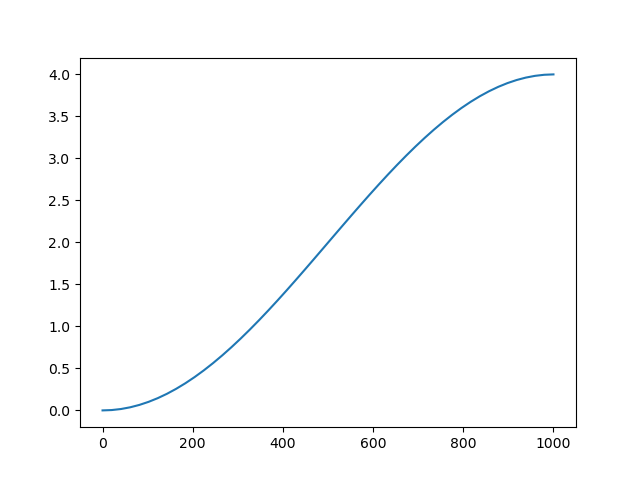
\includegraphics[scale=0.45]{1000_1.png}
    \caption{本征值-自由度解析图像}
\end{figure} 
与图9
 \begin{figure}[H]
        
    \centering
    \vspace{2mm}
    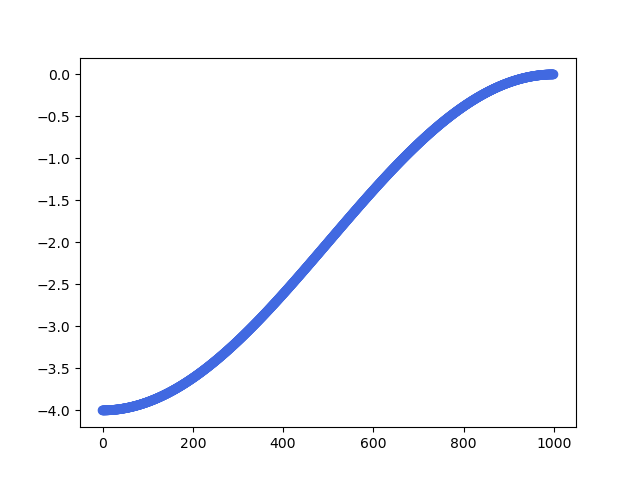
\includegraphics[scale=0.45]{v-1000.png}
\end{figure} 
完美匹配。

至此,我们基本可以认为本次课题计算结果正确。
\newpage
\section{总结}
本次课题首先以五自由度的微振动系统的问题的数值探究
入手,复现出前人的进展,接下来进行理论推广,得到了
多自由度的微振动系统的本征问题的数值计算。期间进行了时间复杂度的
多次优化和算法改进,最终得到的计算结果和理论值匹配,
并认为本课题程序计算结果较为准确,
可以进行固定边界条件下一维原子链的集体振动行为
数值模拟。





\newpage

\begin{thebibliography}{99}
    \bibitem{a}William H. Press, Saul A. Teukolsky, William T. Vetterling, Brian P. Flannery. \emph{Numerical recipes the art of scientific computing },Cambridge University Press[M]2010 \ ISBN:9780521308113
    \bibitem{b} Roberto Tamassia , Michael H. Goldwasser , Michael T. Goodrich  \emph{Data Structures and Algorithms in Python}[M]. Wiley Press ISBN:978-1118290279
    \bibitem{c}彭芳麟. \emph{计算物理基础}[M]. 高等教育出版社\ \ 2010\ \ ISBN\ :\ 9787040283556 
    \bibitem{e}Steven E.Koonin \emph{Computational Physics}[M]Westview Press ISBN: 9780201386233 
    \bibitem{f}Wikipedia.\emph{Iterative method}
    \bibitem{g}zhihu. \emph{固定边界条件与周期边界条件下一维原子链的集体振动行为}
    \bibitem{h}刘川. \emph{理论力学}[M].北京大学出版社.\ \ 2019\ \ ISBN:9787301306536
    \bibitem{i}朗道. \emph{力学}[M].ISBN:9787040208498
\end{thebibliography}

\newpage
\section{附录}
\begin{appendices}
    \renewcommand{\thesection}{\Alph{section}}
    \subsection{全部程序实现}
    \subsubsection{$Gerschgorin$圆盘}
        {    \begin{flushright}
    \scriptsize\emph{运行环境\\$Ubuntu 9.3.0-17\ Ubuntu1~20.04LTS$}\\
    \scriptsize\emph{$Python 3.8.8$\ \ $Anaconda 4.10.3\ \  AMD-4800u$}
        
    \end{flushright}
    \inputpython{Gerschgorin-plt.py}{1}{35}

    }
    \subsubsection{5自由度+画图+模式图}
    {    \begin{flushright}
        \scriptsize\emph{运行环境\\$Ubuntu 9.3.0-17\ Ubuntu1~20.04LTS$}\\
        \scriptsize\emph{$Python 3.8.8$\ \ $Anaconda 4.10.3\ \  AMD-4800u$}
            
        \end{flushright}
        \inputpython{5_pic.py}{1}{144}
    
        }
        \subsubsection{N自由度}
    {    \begin{flushright}
        \scriptsize\emph{运行环境\\$Ubuntu 9.3.0-17\ Ubuntu1~20.04LTS$}\\
        \scriptsize\emph{$Python 3.8.8$\ \ $Anaconda 4.10.3\ \  AMD-4800u$}
            
        \end{flushright}
        \inputpython{fin_n.py}{1}{119}
    
        }
        \subsubsection{N自由度+画图(用numpy本征值函数)}
        {    \begin{flushright}
            \scriptsize\emph{运行环境\\$Ubuntu 9.3.0-17\ Ubuntu1~20.04LTS$}\\
            \scriptsize\emph{$Python 3.8.8$\ \ $Anaconda 4.10.3\ \  AMD-4800u$}
                
            \end{flushright}
            \inputpython{n_yes.py}{3}{155}
        
            }
            \subsubsection{N自由度+画图(未用numpy本征值函数)}
            {    \begin{flushright}
                \scriptsize\emph{运行环境\\$Ubuntu 9.3.0-17\ Ubuntu1~20.04LTS$}\\
                \scriptsize\emph{$Python 3.8.8$\ \ $Anaconda 4.10.3\ \  AMD-4800u$}
                    
                \end{flushright}
                \inputpython{n_no.py}{3}{145}
            
                }
                \subsubsection{驻波画图}
            {    \begin{flushright}
                \scriptsize\emph{运行环境\\$Ubuntu 9.3.0-17\ Ubuntu1~20.04LTS$}\\
                \scriptsize\emph{$Python 3.8.8$\ \ $Anaconda 4.10.3\ \  AMD-4800u$}
                    
                \end{flushright}
                \inputpython{2000_paintzhubo.py}{3}{183}
            
                }
                \subsubsection{本征值-自由度解析画图}
                {    \begin{flushright}
                    \scriptsize\emph{运行环境\\$Ubuntu 9.3.0-17\ Ubuntu1~20.04LTS$}\\
                    \scriptsize\emph{$Python 3.8.8$\ \ $Anaconda 4.10.3\ \  AMD-4800u$}
                        
                    \end{flushright}
                    \inputpython{2000_jiei.py}{1}{9}
                
                    }

    \renewcommand{\thesection}{\Alph{section}}
    \subsection{固定边界条件下的一维原子链的集体振动模式的推导}
{
    在简谐近似下,一维原子链可简化为如课题探究的模型,
    细绳的倔强系数为k(根据题目,k=1),振子的质量为m,体系的总振子数目为N(自由度)。
易见,体系的拉氏量可写成:

\begin{equation}
    \mathscr{L}=\sum_{i} \frac{1}{2} m \dot{x}_{l}-\frac{1}{2} k\left[x_{1}^{2}+\left(x_{2}-x_{1}\right)^{2}+\cdots+\left(x_{N}-x_{N-1}\right)^{2}+x_{N}^{2}\right]
    \end{equation}

    那么下面我们来求解一下这个体系的简正模与简正频率:
\begin{equation*}
        \normalsize{
        \begin{aligned}
        L&=\sum_{i=1}^{N} \frac{1}{2} m \dot{x}_{i}-\sum_{i=2}^{N} \frac{1}{2} k\left(x_{i}-x_{i-1}\right)^{2}+\frac{1}{2} k\left(x_{N}^{2}-x_{1}^{2}\right) \\
        &=\sum_{i=1}^{N} \frac{1}{2} m \dot{x}_{l}-\sum_{i=2}^{N} \frac{1}{2} k\left(x_{i}^{2}-2 x_{i} x_{i-1}+x_{i-1}^{2}\right)+\frac{1}{2} k\left(x_{N}^{2}-x_{1}^{2}\right) \\
        U&=\sum_{i=2}^{N} \frac{1}{2} k\left(x_{i}^{2}+x_{i-1}^{2}\right)-\sum_{i=2}^{N} k x_{i} x_{i-1}+\frac{1}{2} k\left(x_{N}^{2}-x_{1}^{2}\right) \\
        d U&=\sum_{i=2}^{N} k\left(x_{i} d x_{i}+x_{i-1} d x_{i-1}\right)-\sum_{i=2}^{N} k\left(d x_{i} x_{i-1}+x_{i} d x_{i-1}\right)+k\left(x_{N} d x_{N}-x_{1} d x_{1}\right) \\
        \frac{\partial U}{\partial x_{\alpha}}&=\sum_{i=2}^{N} k\left(x_{i} \frac{\partial x_{i}}{\partial x_{\alpha}}+x_{i-1} \frac{\partial x_{i-1}}{\partial x_{\alpha}}\right)-\sum_{i=2}^{N} k\left(\frac{\partial x_{i}}{\partial x_{\alpha}} x_{i-1}+x_{i} \frac{\partial x_{i-1}}{\partial x_{\alpha}}\right)+k\left(x_{N} \frac{\partial x_{N}}{\partial x_{\alpha}}-x_{1} \frac{\partial x_{1}}{\partial x_{\alpha}}\right) \\
        &=\sum_{i=2}^{N} k\left(x_{i} \delta_{\alpha}^{i}+x_{i-1} \delta_{\alpha}^{i-1}\right)-\sum_{i=2}^{N} k\left(x_{i-1} \delta_{\alpha}^{i}+x_{i} \delta_{\alpha}^{i-1}\right)+k\left(x_{N} \delta_{\alpha}^{N}-x_{1} \delta_{i j}^{1}\right]
        \end{aligned}}
        \end{equation*}

        由上式可知:

        (1)当 $\alpha=1$ 时
        $$
        \frac{\partial U}{\partial x_{\alpha}}=k x_{1}-k x_{2}-k x_{1}=-k x_{2}
        $$

        (2)当 $\alpha=N$ 时
        $$
        \frac{\partial U}{\partial x_{\alpha}}=k x_{N}-k x_{N-1}-k x_{N}=2 k x_{N}-k x_{N-1}
        $$

        (3)当 $\alpha=2,3,4, \ldots, N-1$ 时
        $$
        \frac{\partial U}{\partial x_{\alpha}}=k x_{\alpha}+k x_{\alpha}-k x_{\alpha-1}-k x_{\alpha+1}=k\left(2 x_{\alpha}-x_{\alpha-1}-x_{\alpha+1}\right)
        $$

因此对于 $\frac{\alpha^{2} U}{\alpha x_{\alpha} \alpha x_{\beta}}$ 有:
(1)当 $\alpha=1, \beta=2$ 时
$$
\frac{\partial^{2} U}{\partial x_{\alpha} \alpha x_{\beta}}=-k
$$

(2)当 $\alpha=1, \beta \neq 2$ 时
$$
\frac{\partial^{2} U}{\partial x_{\alpha} \partial x_{\beta}}=0
$$

(3)当 $\alpha=N, \beta=N$
$$
\frac{\partial^{2} U}{\partial x_{\alpha} \partial x_{\beta}}=2 k
$$

(4)当 $\alpha=N, \beta=N-1$ 时
$$
\frac{\partial^{2} U}{\partial x_{\alpha} \partial x_{\beta}}=-k
$$

(5) $\alpha=N, \beta \neq N$ 或 $N-1$ 时
$$
\frac{\partial^{2} U}{\partial x_{\alpha} \partial x_{\beta}}=0
$$

(6)当 $\alpha=2,3,4, \ldots, N-1$ 时
$$
\frac{\partial^{2} U}{\partial x_{\alpha} \partial x_{\beta}}=k\left(2 \delta_{\beta}^{\alpha}-\delta_{\beta}^{\alpha-1}-\delta_{\beta}^{\alpha+1}\right)
$$

综上所述, $\hat{U}=\left[\frac{\partial^{2} U}{\partial x_{\alpha} \partial x_{\beta}}\right]_{\alpha \beta}$ 矩阵可写为
$$
\hat{U}=k\left[\begin{array}{cccccc}
2 & -1 & 0 & \cdots & \cdots & \\
-1 & 2 & -1 & \ddots & & \\
0 & -1 & 0 & & \ddots & \\
0 & & \ddots & \ddots & & \\
\vdots & & & \ddots & \ddots & -1
\end{array}\right]_{N X N}
$$
而又因 $T=\frac{1}{2} \sum_{i} m_{i k} \dot{x}_{l} \dot{x}_{k}=\sum_{i=1}^{N} \frac{1}{2} m \dot{x}_{l}$
$\therefore \hat{M}=\left[m_{i k}\right]_{i k}$ 矩阵可写为
$$
\hat{M}=m\left[\begin{array}{ccccc}
1 & & & & \\
& 1 & & & \\
& & 1 & & \\
& & & \ddots & \\
& & & & 1
\end{array}\right]
$$
于是体系的久期方程为 $\operatorname{det}\left(-w^{2} \hat{M}+\hat{U}\right)=0$, 即

$$
\left[\begin{array}{cccc}
2 k-w^{2} m & -k & \ldots & \\
-k & 2 k-w^{2} m & -k & \ldots \\
0 & -k & 2 k-w^{2} m & \\
\vdots & \vdots & &
\end{array}\right]_{N \times N}=0 \text { (在后面的推导中, 我们将该行列记为 } D_{N} \text { ) }
$$

易发现久期方程为一个三对角矩阵的行列式, 将其按第一行展开有:
$$
D_{N}=\left(2 k-w^{2} m\right) D_{N-1}-k^{2} D_{N-2} \cdots \cdots
$$
其中 $D_{1}=2 k-w^{2} m, D_{2}=\left|\begin{array}{cc}2 k-w^{2} m & -k \\ -k & 2 k-w^{2} m\end{array}\right|=\left(2 k-w^{2} m\right)-k^{2}$ 引入待定参数 $\alpha$ 和 $\beta$, 满足:
$$
\alpha+\beta=2 k-w^{2} m, \alpha \beta=k^{2}\left(\alpha+\beta=D_{1}, \alpha \beta=D_{1}^{2}-D_{2}\right)
$$
使 (1) 式变为:
$$
D_{N}-\alpha D_{N-1}=\beta\left(D_{N-1}-\alpha D_{N-2}\right) \cdots \cdots
$$
为求参数 $\alpha$ 和 $\beta$, 令:
$$
\lambda^{2}-\left(2 k-w^{2} m\right) \lambda+k^{2}=0
$$
上式即为本征方程, 而 $\alpha 、 \beta$ 为期的两根
计算本征方程的判别式, 有:
$$
\Delta=b^{2}-4 a c=\left(2 k-w^{2} m\right)^{2}-4 k^{2}=\left(2 k-w^{2} m\right)^{2}-(2 k)^{2}<0
$$
因此, 本征方程有两个互为共轭的复根:

$$
\begin{aligned}
&\alpha=\frac{1}{2}\left(2 k-w^{2} m\right)+i \frac{1}{2} \sqrt{-\Delta} \\
&\beta=\frac{1}{2}\left(2 k-w^{2} m\right)-i \frac{1}{2} \sqrt{-\Delta}
\end{aligned}
$$
注意到 $\alpha$ 和 $\beta$ 实际上地位是价位的, 因此 (2) 式可写为
$$
\left\{\begin{array}{l}
D_{N}-\alpha D_{N-1}=\beta\left(D_{N-1}-\alpha D_{N-2}\right) \ldots \ldots \\
D_{N}-\beta D_{N-1}=\alpha\left(D_{N-1}-\beta D_{N-2}\right) \ldots \ldots
\end{array}\right.
$$
(3) 式告诉我们, $\left\{D_{N}-\alpha D_{N-1}\right\}$ 是以 $\beta$ 为公比的等比数列, 因此有:
$$
D_{N}-\alpha D_{N-1}=\beta^{N-2}\left(D_{2}-\alpha D_{1}\right) \cdots \cdots
$$
同样, (4) 式告诉我们, $\left\{D_{N}-\beta D_{N-1}\right\}$ 是以 $\alpha$ 为公比的等比数列, 因此有:
$$
D_{N}-\beta D_{N-1}=\alpha^{N-2}\left(D_{2}-\beta D_{1}\right) \cdots \cdots
$$
联立 (5)、(6) 式, 消去 $D_{N-1}$ 得:
$$
\begin{gathered}
D_{N}-\beta D_{N-1}=\alpha^{N-2}\left(D_{2}-\beta D_{1}\right) \\
D_{N}=\frac{1}{\alpha-\beta}\left[\alpha^{N-1}\left(D_{2}-\beta D_{1}\right)-\beta^{N-1}\left(D_{2}-\alpha D_{1}\right)\right] \\
=\frac{1}{\alpha-\beta}\left[\alpha^{N-1} D_{2}-\alpha^{N-1} \beta D_{1}-\beta^{N-1} D_{2}+\beta^{N-1} \alpha D_{1}\right] \\
=\frac{1}{\alpha-\beta}\left[D_{2}\left(\alpha^{N-1}-\beta^{N-1}\right)+D_{1}\left(\alpha \beta^{N-1}-\beta \alpha^{N-1}\right)\right] \\
\because \alpha+\beta=D_{1}, \alpha+\beta=D_{1}^{2}-D_{2} \\
\therefore D_{2}=D_{1}^{2}-(\alpha+\beta)=(\alpha+\beta)^{2}-(\alpha+\beta)=\alpha^{2}+\beta^{2}+\alpha \beta \\
\therefore D_{N}=\frac{1}{\alpha-\beta}\left[\left(\alpha^{2}+\beta^{2}+\alpha \beta\right)\left(\alpha^{N-1}-\beta^{N-1}\right)+(\alpha+\beta)\left(\alpha \beta^{N-1}-\beta \alpha^{N-1}\right)\right]
\end{gathered}
$$
化简后有
$$
D_N=\frac{1}{\alpha-\beta}\left[D_{2}\left(\alpha^{N-1}-\beta^{N-1}\right)+D_{1}\left(\alpha \beta^{N-1}-\beta \alpha^{N-1}\right)\right]
$$
同时
$$
\begin{aligned}
&\because \alpha+\beta=D_{1}, \alpha+\beta=D_{1}^{2}-D_{2} \\
&\therefore D_{2}=D_{1}^{2}-(\alpha+\beta)=(\alpha+\beta)^{2}-(\alpha+\beta)=\alpha^{2}+\beta^{2}+\alpha \beta \\
&\begin{aligned}
\therefore D_{N} &=\frac{1}{\alpha-\beta}\left[\left(\alpha^{2}+\beta^{2}+\alpha \beta\right)\left(\alpha^{N-1}-\beta^{N-1}\right)+(\alpha+\beta)\left(\alpha \beta^{N-1}-\beta \alpha^{N-1}\right)\right] \\
&=\frac{1}{\alpha+\beta}\left[\left(\alpha^{N+1}-\alpha^{2} \beta^{N-1}+\beta^{2} \alpha^{N-1}-\beta^{N+1}+\alpha^{N} \beta-\alpha \beta^{N}\right)+\alpha^{2} \beta^{N-1}-\beta \alpha+\alpha \beta^{N}\right.\\
&\left.-\beta^{2} \alpha^{N-1}\right]
\end{aligned} \\
&\quad=\frac{1}{\alpha+\beta}\left(\alpha^{N+1}-\beta^{N-1}\right)
\end{aligned}
$$
$$
\text { 令 } \alpha=r e^{i \theta} 、 \beta=r e^{-i \theta}
$$
则久期方程可化为:
$$
\begin{aligned}
&\quad \therefore e^{i(2 N+2) \theta}=1 \\
&\therefore \theta_{n}=\frac{n}{N+1} \pi(n=1,2,3 \ldots N) \\
&\because \alpha=\frac{1}{2}\left(2 k-w^{2} m\right)+i \frac{1}{2} \sqrt{4 k^{2}-\left(2 k-w^{2} m\right)^{2}} \\
&\therefore \tan \theta_{n}=\frac{\sqrt{4 k^{2}-\left(2 k^{2}-w_{n}^{2} m\right)^{2}}}{2 k-w_{n}^{2} m} \\
&\therefore\left(2 k^{2}-w_{n}^{2} m\right)^{2} \tan ^{2} \theta_{n}=4 k^{2}-\left(2 k^{2}-w_{n}^{2} m\right)^{2} \\
&\therefore\left(2 k^{2}-w_{n}^{2} m\right)^{2}\left(\tan ^{2} \theta_{n}+1\right)=4 k^{2} \\
&\therefore\left(2 k^{2}-w_{n}^{2} m\right)^{2}=\frac{4 k^{2}}{\tan ^{2} \theta_{n}+1} \\
&\therefore 2 k^{2}-w_{n}^{2} m=\pm 2 k \cdot\left(\tan ^{2} \theta_{n}+1\right)^{-\frac{1}{2}} \\
&\therefore w_{n}^{2}=\frac{2 k}{m}\left[1 \pm\left(\tan ^{2} \theta_{n}+1\right)^{-\frac{1}{2}}\right]\left(\theta_{n}=\frac{n}{N+1} \pi, n=1,2,3 \ldots N\right) \\
&\because \tan ^{2} \theta_{n}+1=\frac{1}{\cos ^{2} \theta_{n}}
\end{aligned}
$$
$\therefore w_{n}^{2}=\frac{2 k}{m}\left[1-\cos \theta_{n}\right]$ (此处将士取作 “-” 的原因为 $\theta_{n} \in(0, \pi)$, 因此 “-” 包含了 “+” 所有情况)
$$
\because \hat{M}=m \cdot \hat{I}
$$
$\therefore$ 对于体系的简正模, 我们只需考虑 $\hat{U}$ 的本征向量即可 猜测与 $w_{n}$ 相应的简正模的形式为
$$
\left[\sin \frac{n \pi}{N+1}, \sin \frac{2 n \pi}{N+1}, \sin \frac{3 n \pi}{N+1}, \ldots \ldots, \sin \frac{N n \pi}{N+1}\right]^{T}
$$
此简正模的形式相当于驻波( $\mathrm{y}=\mathrm{y} 1+\mathrm{y} 2=2 \operatorname{Acos} 2 \pi(\mathrm{x} / \lambda) \cos 2 \pi(\mathrm{t} / \mathrm{T}))$, 所以在固定边界条 件下猜此解是合理的。
我们不妨代入验证:
$$
k\left[\begin{array}{ccccc}
2 & -1 & 0 & \cdots & \cdots \\
-1 & 2 & -1 & 0 & \cdots \\
0 & -1 & 2 & -1 & \\
\vdots & \vdots & \vdots & \ddots & \\
& & & \ddots
\end{array}\right]_{N X N}\left[\begin{array}{c}
\sin \frac{n \pi}{N+1} \\
\sin \frac{2 n \pi}{N+1} \\
\sin \frac{3 n \pi}{N+1} \\
\vdots \\
\sin \frac{N}{N+1} n \pi
\end{array}\right]=k\left[\begin{array}{c}
2 \sin \frac{n \pi}{N+1}-\sin \frac{2 n \pi}{N+1} \\
-\sin \frac{n \pi}{N+1}+2 \sin \frac{2 n \pi}{N+1}-\sin \frac{3 n \pi}{N+1} \\
\frac{2 n \pi}{N+1}+2 \sin \frac{3 n \pi}{N+1}+\sin \frac{4 n \pi}{N+1} \\
\vdots \\
-\sin \frac{(N-1)}{(N+1)} n \pi+2 \sin \frac{N}{N+1} n \pi
\end{array}\right]
$$

$$
2 \sin \frac{n \pi}{N+1}-2 \sin \frac{n \pi}{N+1} \cos \frac{n \pi}{N+1}=2 \sin \frac{n \pi}{N+1}\left(1-\cos \frac{n \pi}{N+1}\right)
$$
$$
\begin{aligned}
&-\sin \frac{n \pi}{N+1}+2 \sin \frac{2 n \pi}{N+1}-\sin \frac{3 n \pi}{N+1}\\
&=-\sin \frac{n \pi}{N+1}+2 \sin \frac{2 n \pi}{N+1}-\left(\sin \frac{2 n \pi}{N+1} \cos \frac{n \pi}{N+1}+\sin \frac{n \pi}{N+1} \cos \frac{2 n \pi}{N+1}\right)\\
&=-\sin \frac{n \pi}{N+1}-\sin \frac{n \pi}{N+1} \cos \frac{2 n \pi}{N+1}+2 \sin \frac{2 n \pi}{N+1}-\sin \frac{2 n \pi}{N+1} \cos \frac{n \pi}{N+1}\\
&=\left(-\sin \frac{n \pi}{N+1}-\sin \frac{n \pi}{N+1} \cos \frac{2 n \pi}{N+1}+\sin \frac{2 n \pi}{N+1} \cos \frac{n \pi}{N+1}\right)+2 \sin \frac{2 n \pi}{N+1}\left(1-\cos \frac{n \pi}{N+1}\right)\\
&=\left[-\sin \frac{n \pi}{N+1}-\sin \frac{n \pi}{N+1}\left(2 \cos ^{2} \frac{2 n \pi}{N+1}-1\right)+2 \sin \frac{n \pi}{N+1} \cos ^{2} \frac{n \pi}{N+1}\right]+2 \sin \frac{2 n \pi}{N+1}(1\\
&\left.-\cos \frac{n \pi}{N+1}\right)\\
&=2 \sin \frac{2 n \pi}{N+1}\left(1-\cos \frac{n \pi}{N+1}\right)\\
&-\sin \frac{N-1}{N+1} n \pi+2 \sin \frac{N}{N+1} n \pi\\
&=-\left[\sin \frac{N}{N+1} n \pi \cos \frac{1}{N+1} n \pi-\sin \frac{1}{N+1} n \pi \cos \frac{N}{N+1} n \pi\right]+2 \sin \frac{N}{N+1} n \pi\\
&=-\left[\sin \frac{N}{N+1} n \pi \cos \frac{1}{N+1} n \pi-\sin \frac{1}{N+1} n \pi \cos \frac{N}{N+1} n \pi-2 \sin \frac{N}{N+1} n \pi \cos \frac{1}{N+1} n \pi\right]\\
&+2 \sin \frac{N}{N+1} n \pi-2 \sin \frac{N}{N+1} n \pi \cos \frac{1}{N+1} n \pi\\
&=\left[-\sin \frac{1}{N+1} n \pi \cos \frac{N}{N+1} n \pi-\sin \frac{N}{N+1} n \pi \cos \frac{1}{N+1} n \pi\right]+2 \sin \frac{N}{N+1} n \pi(1\\
&\left.-2 \cos \frac{n}{N+1} \pi\right)\\
&=-\sin \frac{N+1}{N+2} n \pi+2 \sin \frac{N}{N+1} n \pi\left(1-2 \cos \frac{n}{N+1} \pi\right)
\end{aligned}
$$

$$
\therefore k\left[\begin{array}{ccc}
2 & -1 & \cdots \\
-1 & 2 & \cdots \\
\vdots & & \ddots
\end{array}\right]_{N X N}\left[\begin{array}{c}
\sin \frac{n \pi}{N+1} \\
\sin \frac{2 n \pi}{N+1} \\
\vdots \\
\sin \frac{N}{N+1} n \pi
\end{array}\right]=2 k\left(1-\cos \frac{n}{N+1} \pi\right)\left[\begin{array}{c}
\sin \frac{n \pi}{N+1} \\
\sin \frac{2 n \pi}{N+1} \\
\vdots \\
\sin \frac{N}{N+1} n \pi
\end{array}\right]
$$
即, 向量 $$\left[\sin \frac{n \pi}{N+1}, \sin \frac{2 n \pi}{N+1}, \sin \frac{3 n \pi}{N+1}, \ldots \ldots, \sin \frac{N n \pi}{N+1}\right]^{T}$$ 确实为体系的简正模,其所对应的简 正频率为 $$w_{n}^{2}=\frac{2 k}{m}\left(1-\cos \theta_{n}\right)\left(\theta_{n}=\frac{n}{N+1} \pi, n=1,2,3 \ldots N\right)$$.
}

\end{appendices}

\end{document}